\section{Analisi di Fourier}
L'analisi di Fourier decompone il segnale in costituenti sinusoidali di differenti frequenze. Il segnale non è più nel dominio tempo-spazio, ma delle frequenze: i dati sono gli stessi, cambia solo la rappresentazione.

\textit{Ogni funzione periodica e a quadrato sommabile può essere espressa come somma infinita e pesata di funzioni seno e coseno (combinazioni di funzioni armoniche).}

Si ricorda che una sequenza periodica è $x(n) = x(n + T)$. Una funzione armonica è una funzione periodica del tipo:
$$y = A\sin(\varpi x + \varphi) \qquad y = A\cos(\varpi x + \varphi)$$
Dove $A$ è l'ampiezza, $\varpi$ è la pulsazione, $\varphi$ è la fase. Si ha che $\varpi = 2\pi/T$ dove $1/T$ è la frequenza, e $\pi$ è $180^{\circ}$.

Sviluppando i seni e i coseni si ha, con $a = A\sin(\varphi)$ e $b = A\cos(\varphi)$: \\
$y = A\sin(\varpi x + \varphi) = a\cos (\varpi x) + b\sin(\varpi x)$ \\
$y = A\cos(\varpi x + \varphi) = b\cos(\varpi x) + a\sin(\varpi x)$ \\

Le armoniche vengono combinate una per volta, avvicinandosi man mano alla funzione originaria.
\begin{figure}[h]
	\centering
	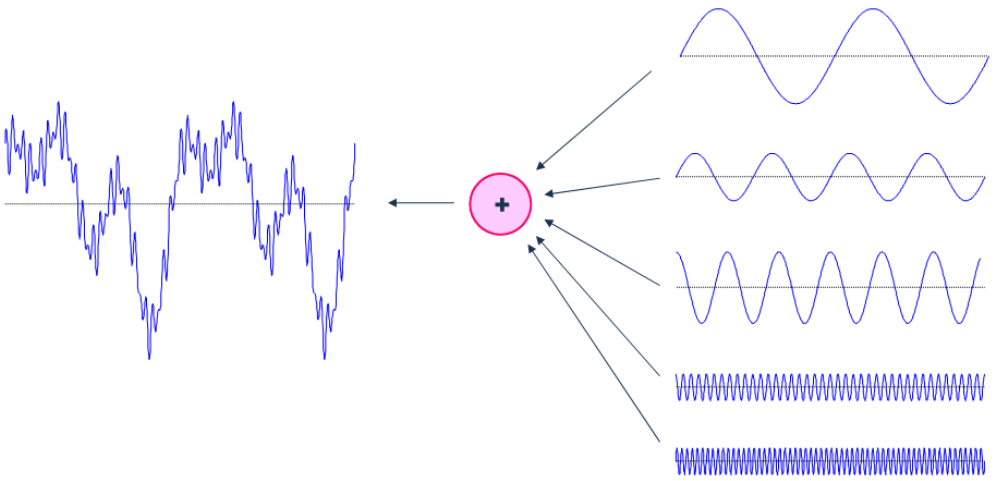
\includegraphics[scale=0.43]{Lezioni/Immagini/fourier}
\end{figure}

\subsection{Serie di Fourier}
La serie di Fourier è una formula utile per approssimare la scomposizione. Rappresenta una funzione periodica mediante combinazione lineare di funzioni sinusoidali.
$$f(x) = \frac{a_0}{2} + \sum_{k=1}^{\infty} a_k \cos\Big(\frac{2\pi}{N}kx\Big) + b_k\sin\Big(\frac{2\pi}{N}kx\Big)$$
$$N \rightarrow \text{periodo} \qquad (1/N) \rightarrow \text{frequenza fondamentale } f_0 \qquad (1/N)k \rightarrow \text{frequenze multiple } kf_0$$

$a_k$ e $b_k$ sono numeri reali, $k$ è un numero intero che funge da fattore moltiplicativo e $N$ è l'ampiezza della parte di funzione che si ripete periodicamente (l'inverso è la frequenza fondamentale). $x$ è la variabile indipendente.

Le frequenze (infinite), quindi, sono una parte fondamentale della formula. Con tempo $T = 1/f$ il dominio del tempo è $t$, e il dominio della frequenza è $Hz$. In altre parole, il segnale passa dal dominio spazio-tempo alle frequenze, con coppie frequenza-peso associate alla sinusoidale (ampia $A$).

Estendendo la formula con il concetto di pulsazione, si ha che una pulsazione è $\varpi_k = 2\pi f_k$, e di conseguenza:
$$f(x) = \frac{a_0}{2} + \sum_{k=1}^{\infty} a_k \cos(2\pi kf_0x) + b_k\sin(2\pi kf_0x)$$
$$a_k = \frac{2}{N} \int_{-\frac{N}{2}}^{\frac{N}{2}} f(x)\cos(2\pi kf_0x) dx \qquad b_k = \frac{2}{N} \int_{-\frac{N}{2}}^{\frac{N}{2}} f(x)\sin(2\pi kf_0x) dx$$

La variabile $x$ e la funzione associata sono continue (periodiche), ma la variabile di frequenza è discreta ($k$ intera), quindi dall'integrale si passa alla sommatoria.

Si ricorda che $N$ è il periodo. Data la funzione $f(x)$ periodica, i coefficienti della serie sono \textbf{univocamente} determinati. I coefficienti sono i fattori moltiplicativi di seno e coseno, in relazione al tempo $t$.

Questo significa che esiste biunivocità, la trasformazione può essere effettuata da entrambi i versi senza perdere informazione.

\subsection{Fourier e i suoni}
I suoni elementari hanno andamento sinusoidale, periodico e con estensione indefinita; la maggior parte dei suoni in natura sono però caratterizzati da forme d'onda diverse.

\begin{wrapfigure}{R}{0.44\textwidth}
	\vspace{-15pt}
	\begin{center}
		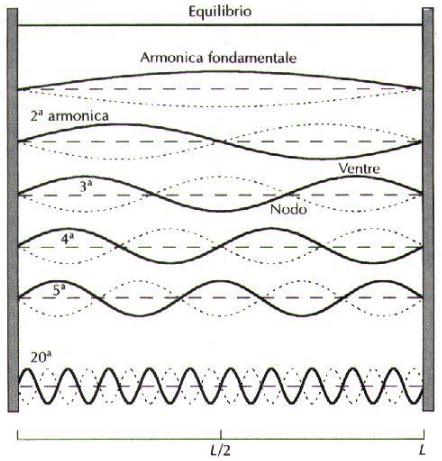
\includegraphics[width=0.4\textwidth]{Lezioni/Immagini/armoniche}
	\end{center}
	\vspace{-50pt}
\end{wrapfigure}

Un segnale si definisce complesso quando è formato da più funzioni sinusoidali combinate, invece che una sola.

Si può dimostrare che, fatte alcune ipotesi di regolarità sull'andamento della forma d'onda, un generico suono complesso può essere descritto come una combinazione di suoni elementari (armoniche).

Le armoniche sono funzioni che, combinate fra loro, permettono di determinare il timbro degli strumenti musicali. Insieme costituiscono forme d'onda. 

\subsection{Onda quadra}
L'onda quadra è un caso particolare in cui tutte le armoniche pari sono nulle, e l'onda quadra è data dalla forma delle componenti $F_0, 3F_0, 5F_0, \dots$ cioè 200 Hz, 600 Hz, 1 Kz eccetera. Si ricorda che l'ampiezza di conseguenza è $\nicefrac{1}{3}, \nicefrac{1}{5}, \dots$ cioè la parte dispari della sommatoria.

Ognuna di queste componenti ha un'ampiezza diversa rispetto a quella dell'armonica fondamentale. La funzione è asimmetrica, e i termini pari sono appunto i coseni: ci sono solo seni non nulli. 

\begin{wrapfigure}{L}{0.48\textwidth}
	\vspace{-5pt}
	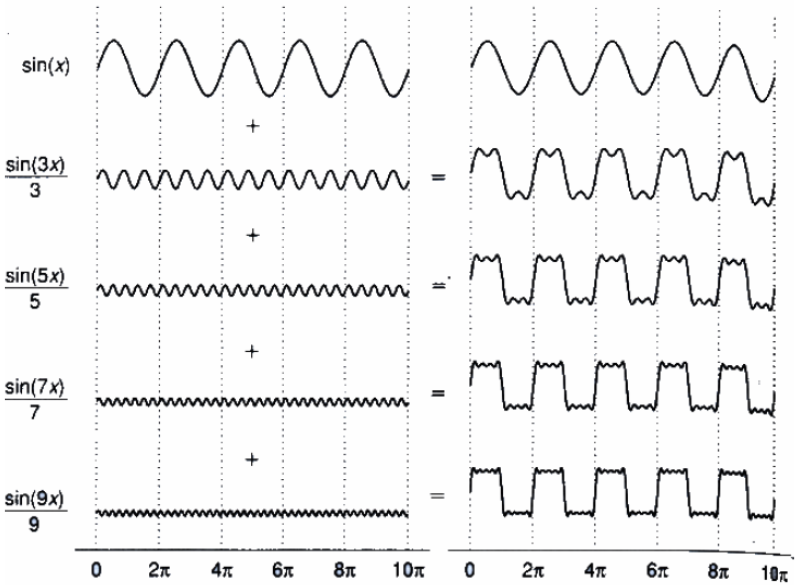
\includegraphics[width=0.45\textwidth]{Lezioni/Immagini/ondaquadra}
	\vspace{-25pt}
\end{wrapfigure}

Esempio: un'onda quadra con periodo 5 ms può essere ottenuta sommando onde sinusoidali di opportuna frequenza, ampiezza e fase. Il contributo più rilevante è dato dalla prima sinusoide, si frequenza pari a quella dell'onda quadra (200 Hz, frequenza fondamentale $F_0$).

Per costruire l'onda quadra sono necessarie anche altre componenti elementari di frequenza maggiore, le armoniche multiple di $F_0$. \\

\subsection{Numeri complessi e serie di Fourier}
I numeri complessi sono rappresentabili su un piano cartesiano come l'intersezione tra numeri reali sull'asse $x$ e numeri complessi sull'asse $y$. Ogni numero complesso ha quindi una parte reale $a$ e una immaginaria $b$.
$$z = ai+b \qquad \abs{z} = \sqrt{a^2 + b^2} = \pi$$

\begin{wrapfigure}{I}{0.43\textwidth}
	\vspace{-15pt}
		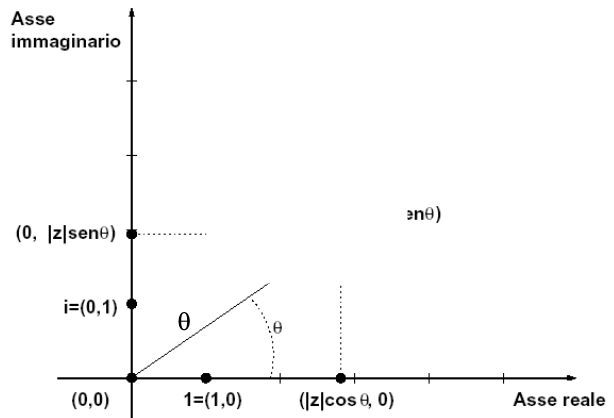
\includegraphics[width=0.42\textwidth]{Lezioni/Immagini/cartesiano}
	\vspace{-30pt}
\end{wrapfigure}

Forma polare:  \\ 
$a = \pi\cos(\theta)$ \\ 
$b = \pi\sin(\theta)$ \\ 
$\theta = \arctan\Big(\frac{b}{a}\Big)$

Le coordinate polari corrispondono a quelle cartesiane (proiezione). 

Applicando i numeri complessi alla serie di Fourier e quindi cambiando dominio, si possono usare gli esponenziali complessi e la formula di Eulero. 
$$e^{j\theta} = \cos\theta + j\sin\theta \qquad e^{-j\theta} = \cos\theta - j\sin\theta$$
Sia seno che coseno sono somme di due esponenziali complessi, con segno $+$ e $-$ rispettivamente. Il picco della frequenza è intero per il coseno, immaginario per il seno. 
$$\cos\theta = \frac{1}{2}(e^{j\theta} + e^{-j\theta}) \qquad \sin\theta = -\frac{j}{2}(e^{j\theta} - e^{-j\theta})$$
La parte del seno è immaginaria, il coseno è reale. Le formule sono le stesse, ma applicate al sovrainsieme dei complessi $\mathbb{C}$ ($j$ e $i$ sono indicatori convenzionali della parte immaginaria).

Mettendo a sistema seno e coseno ottenuti in questo modo, si può estendere la serie di Fourier rappresentando le somme di contributi nello spazio degli esponenziali complessi.
$$f(x) = \frac{a_0}{2} + \sum_{k=1}^{\infty} a_k \cos(2\pi f_kx) + b_k\sin(2\pi f_kx)$$
$$f(x) = \sum_{-\infty}^{\infty} R_ke^{j(2\pi f_kx)}$$

Si ricorda che $\theta = 2\pi f_k$. Quando $\theta$ cambia segno, l'angolo si sposta. Essendo il coseno pari, questo non cambia; il seno è dispari quindi è l'opposto. 

Per passare dalle variabili discrete alle continue, si usa il coefficiente $R_k$ che raccoglie le due sommatorie (fino a infinito da entrambi i versi) e si applica l'integrale. 
$$R_k = \int_{-\frac{N}{2}}^{\frac{N}{2}} f(x)e^{-j(2\pi f_kx)} dx$$
Il coefficiente $\frac{A_n}{2}$ (altezza del segnale sull'asse $y$) è dato appunto dalla divisione del coefficiente $R$ in 2 parti, seno e coseno: l'ampiezza sarà la metà, e ogni ampiezza viene sommata insieme alle funzioni. C'è corrispondenza biunivoca fra dominio temporale e dominio delle frequenze. I seni hanno solo la parte complessa.

\subsection{Trasformata di Fourier di funzioni continue}
Per passare dalle funzioni periodiche a quelle reali, la sommatoria diventa un integrale. La trasformata di Fourier serve per rapppresentare le funzioni continue come sinusoidi.

Ogni funzione continua $f(x)$ anche se non periodica (purché abbia area finita) può essere espressa come integrale di sinusoidi complesse opportunamente pesate. L'antitrasformata ha dominio spaziale (temporale, diretto) mentre la trasformata ha dominio delle frequenze.
$$\text{Antitrasformata di Fourier: } f(x) = \int_{-\infty}^{\infty} F(u)e^{j2\pi ux} dx$$
$$\text{Trasformata di Fourier: } F(u) = \int_{-\infty}^{\infty} f(x)e^{-j2\pi ux} dx$$
$F(u)$ sostituisce il coefficiente discreto $R_k$, $u$ è la frequenza. La trasformata di Fourier non si può applicare a tutte le funzioni, ma solo a quelle con quadrato sommabile (trovare la formula) e continue.

Dalla trasformata di Fourier, la funzione originiaria può essere ricostruita senza perdita di informazione attraverso il processo inverso: è possibile spostarsi dal dominio spaziale a quello delle frequenze e poi tornare indietro senza aver perso informazione.

Esiste un valore della trasformata (non più $\delta$) per ogni funzione continua. Invertendo la funzione, quindi, se è a supporto finito non ci sarà $2\delta$.

Piuttosto che guardare parte reale e immaginaria, si considerano modulo e fase, ricavabili direttamente. Il modulo indica la potenza del segnale, e la fase assicura la biunivocità della corrispondenza. 
$$F(u) = \digamma[f(x)] = \Re(u) + j\Im(u) = \abs{F(u)}e^{j\phi(u)}$$
$$\text{Spettro: } \abs{F(u)} = [\Re(u)^2 + \Im(u)^2]^{\nicefrac{1}{2}}$$
$$\text{Fase: } \phi(u) = \tan^{-1} \Big[\frac{\Im(u)}{\Re(u)}\Big]$$
$$\text{Potenza (densità) spettrale: } \abs{F(u)}^2 = \Re(u)^2 + \Im(u)^2$$
La trasformata di Fourier è un operatore scomponibile, quindi per passare da una dimensione a $n$ semplicemente si applica $n$ volte la formula. In altre parole, si scompone rispetto a una direzione la funzione.

\subsection{Trasformata di Fourier di funzioni discrete}
Il primo step è il campionamento: in questo caso si utilizza la sommatoria, ma la funzione continua è rappresentata da un numero discreto di campioni. La funzione è definita per campioni $i$, e la variabile indipendente $x$ assume valore complesso $i\Delta x$.
$$F(u) = \int_{-\infty}^{+\infty} f(x)e^{-j2\pi ux} dx \Longrightarrow F(u) = \sum_{i=-\infty}^{\infty} f(i)e^{-j2\pi ui\Delta x}$$
Limitando la funzione spazialmente, il passo $\Delta x$ per convenzione diventa $\nicefrac{1}{N}$, e la sommatoria arriva fino a $N - 1$ invece che infinito. $f(i)$ è la funzione campionata (a partire da $f(x)$ continua): la trasformata è periodica. Si ha $f(i) = f(x_0 + i\Delta x)$.
$$F(u) = \frac{1}{N} \sum_{i=0}^{N-1} f(i)e^{-j2\pi u \frac{1}{N}i}$$
Per campionare le funzioni $f(x)$ e $F(u)$ si applicano le trasformate di Fourier discrete (DFT). Il segnale campionato è periodico, quindi la funzione inversa è comunque periodica con distanza $\nicefrac{1}{\Delta x}$. Se il passo tende a 0, la funzione tende a infinito (senza repliche) e viceversa. 

In altre parole, da una funzione campionata $\Delta x = \nicefrac{1}{N}$ si passa a una funzione continua e periodica di periodo $N$. 

Il fattore $\nicefrac{1}{N}$ davanti alla trasformata o all'antitrasformata è un fattore di normalizzazione per il dualismo fra spazio diretto e spazio trasformato. Di conseguenza, $\Delta u = \frac{1}{N\Delta x}$.

Un ragionamento analogo si applica per passare da una dimensione a due: la sommatoria è doppia e si divide per entrambi i fattori di normalizzazione. Entrambe le variabili rispettano la periodicità, cioè $F(u, v) = F(u + M, v + N)$ con $\Delta u = 1/M \Delta x$, $\Delta v = 1/N \Delta y$.

\subsubsection{Elaborazione di immagini}
Il segnale di un'immagine viene scomposto, come visto precedentemente, in modulo e fase. il modulo raccoglie le frequenza di un'immagine, mentre la fase contiene l'informazione posizionale di ogni in un'immagine (le frequenze sono le stesse a prescindere dall'organizzazione spaziale). L'ampiezza $\angle$ contiene informazioni relative alle posizione o meno delle strutture nell'immagine.
$$F(u, v) = \abs{F(u, v)}e^{j\phi(u, v)}$$
I pixel possono assumere valore da 0 a 255, mappati in una trasformata di Fourieri discreta. Data la periodicità e la simmetria dello spettro rispetto all'origine, è possibile scegliere il periodo dello spettro centrato sull'origine $(0, 0)$.

In questo modo, il picco rappresenza la componente continua (valore medio della funzione), e le frequenze crescono allontanandosi dal picco. Per convenzione lo spettro (in alto a sinistra) si trasla in modo da essere al centro, e le alte frequenze sono verso gli angoli esterni.

Il processo è reversibile: l'immagine, di solito sotto forma di segnale, se viene ricostruita dalla trasformata è identica all'originale.

L'istogramma di un'immagine a livelli di grigio è una funzione discreta $h(r_k) = n_k$ dove $r_k$ è il livello di grigio \textit{k}-simo, e $n_k$ è il numero di pixel nell'immagine con intensità $r_k$ (per ogni livello).

Lo spettro è il risultato della trasformata, di cui una parte è reale e una immaginaria. Le circonferenze dal centro raccolgono la maggioranza della potenza spettrale totale, e manipolando lo spettro il risultato dell'inversione sarà differente.

\subsection{Proprietà della trasformata}
La scomponibilità viene utilizzata per cambiare dimensione. \\
Un'altra importante proprietà è la linearità: la trasformata di Fourier applicata a una funzione che è combinazione lineare (somma pesata) di funzioni, il risultato è uguale alla trasformata di Fourier di ogni funzione presa singolarmente. 
$$F(f)x) + g(x) = F(f(x)) + F(g(x)) = F(u) + G(u)$$
La separabilità e la linearità permettono di ridurre la complessità della trasformata.

Vale anche la traslazione nello spazio (tempo), ma solo per la trasformata discreta: una traslazione equivale a una modulazione nelle frequenze con un esponente complesso.
$$F(f(x + x_0)) = e^{j2\pi ux_0} \qquad F^{-1}(F(u \pm \varpi)) = f(x)e^{\pm j2\pi \varpi x}$$
$$\text{Scala: } F(f(ax)) = \frac{1}{\abs{a}} F\Big(\frac{u}{a}\Big) \implies f(\alpha x, \beta y) = \frac{1}{\abs{\alpha \beta}} F\Big(\frac{u}{\alpha}, \frac{v}{\beta}\Big)$$
$$\text{Inversione: } F(f(-x)) = F(-u)$$
La trasformata di una funzione reale gode di simmetria Hermitiana: la parte reale e il modulo sono simmetrici rispetto all'origine, mentre la parte immaginaria e la fase sono antisimmetriche rispetto all'origine.
$$\text{Periodicità (discreta): } F(u) = F(u + M) \implies F(u) = \frac{1}{M} \sum_{x=0}^{M-1} f(x)e^{-j\frac{2\pi}{M}ux} \quad u = 0, \dots, M - 1$$
Altre proprietà sono già state enunciate, come l'esistenza dell'inversa della trasformata discreta, la separabilità e la reversibilità.
$$\text{Valore medio di una trasformata discreta: } F(0) = \frac{1}{M} \sum{x=0}^{M-1} f(x) = \overline{f}(x)$$
$F(u_0)$ è il peso con cui l'onda complessa $e^{j2\pi u_0x}$ di frequenza $u_0$ concorre a formare il segnale $f(x)$. Se $f(x)$ è un'onda complessa di frequenza $u_k$, $F(u)$ sarà 0 per ogni frequenza diversa da $u_k$.
